\documentclass{report}

\usepackage[francais]{babel}
\usepackage[latin1]{inputenc}
\usepackage{xspace}
\usepackage{float}
%\usepackage{here}
\usepackage{geometry}
\usepackage[dvips]{graphicx}
\usepackage[pdftex,
  colorlinks=true,
  pdfstartview=FitV,
  linkcolor=blue,
  citecolor=blue,
  urlcolor=blue]{hyperref}
  
\newcommand{\visidia}{ViSiDiA\xspace}
\newcommand{\berlios}{BerliOs.de\xspace}
\newcommand{\labri}{LaBRI\xspace}

\author{}
\date{}

\title{
  \begin{flushright}
    \begin{Huge}
      \begin{textbf}
        Projet \visidia\\
      \end{textbf}
    \end{Huge}
    \rule{\textwidth}{2mm}\\
    \large\rm{Rapport}\\
    \vspace{2cm}
    \begin{textbf}\\
      \underline{Auteurs}~:\\
      \vspace{0.5cm}
      \sc
      Ammar Aymen\\
      Balan Alexandre\\
      Ben Alaya Ramzi\\
      Bochu Fabien\\
      Bonin �ric\\
      Lafon Julien\\
      \vspace{5mm}
    \end{textbf}
    \rm 6 avril 2007\\
    \vspace{6.25cm}
  \end{flushright}
  \begin{flushleft}
    %\rule{\textwidth}{2mm}\\
    \small
    \underline{Responsable p�dagogique}~: David Renault.\\
    \underline{Responsables scientifiques}~: Mohamed Mosbah et Brahim Hamid.
  \end{flushleft}
}

\begin{document}


\maketitle
\tableofcontents

\chapter*{Introduction}
\addcontentsline{toc}{chapter}{Introduction}
\chapter{Introduction et motivation}

L'algorithmique  distribu�e  devient de  nos  jours  de  plus en  plus
importante au vu des utilisations  possibles sur les r�seaux et autres
syst�mes distribu�s.\\

Cependant,  les  algorithmes  qui   en  d�coulent  sont  difficiles  �
impl�menter, tester et exp�rimenter. C'est dans le but de faciliter la
t�che �  un utilisateur humain que  \visidia a �t� cr��  (voir le site
internet   \cite{visidiaLaBRI}).   Ce   logiciel  a   pour  principale
caract�ristique  de  permettre  la  visualisation,  au  travers  d'une
animation  graphique en  temps  r�el, de  l'ex�cution d'un  algorithme
distribu� sur un graphe donn�.   Cet algorithme peut �tre choisi parmi
une liste, d�velopp� par l'utilisateur ou encore dessin�
gr�ce � des r�gles de r��criture.\\

\visidia  se compose aujourd'hui  de trois  couches. Tout  d'abord une
interface  graphique qui  permet �  l'utilisateur d'interagir  avec le
programme. Elle  permet de cr�er  des r�seaux (graphes)  et d'ex�cuter
des algorithmes  distribu�s afin de  les tester avec  visualisation ou
non. Ensuite, une biblioth�que de  fonctions de haut niveau qui permet
de d�finir des algorithmes distribu�s (envoi, r�ception, traitement de
messages etc...).  Enfin, un simulateur dont le but est de faire le
pont entre les deux autres parties : c'est le centre de \visidia.\\

Les  fonctionnalit�s   que  proposent   \visidia  sont  tout   �  fait
int�ressantes. Malheureusement, l'implantation  actuelle ne permet pas
de faire des tests sur de gros graphes (avec plus de 20 000 noeuds) ce
qui a amen� les chercheurs du LaBRI charg�s de ce projet � proposer un
sujet de  projet de fin d'ann�e �  l'ENSEIRB. Le PFA est  un module de
quatri�me semestre  d'informatique et a pour but  de nous familiariser
avec les m�thodes de travail en  groupe sur des projets de plus longue
dur�e et de plus grande taille que ceux dont nous avons
l'habitude.\\

Notre  but au  cours  des mois  qui  vont suivre  est  de fournir  une
extension  au logiciel.   Cette extension  aura pour  r�le  d'offrir �
l'utilisateur les outils (analogues � ceux existants d�j�) n�cessaires
� l'ex�cution d'algorithmes distribu�s � l'aide d'agents mobiles.\\

Les d�finitions de la notion d'agent mobile sont nombreuses c'est pour
cela  que nous  devons nous  tenir  � le  d�finition plus  restrictive
donn�e par  les clients.  Dans le  cadre de \visidia,  un agent mobile
sera donc une entit� autonome de  calcul qui se d�place dans le graphe
et agit  sur les  noeuds en fonction  de l'algorithme �  ex�cuter. Une
bonne  r�f�rence concernant  ce type  d'agent pourra  se  trouver dans
\cite{agentBook}.

L'implantation  des  agents mobiles  dans  \visidia permettra,  ainsi,
d'augmenter   ses  capacit�s   de  simulation.    Les   deux  m�thodes
(algorithmique  distribu�e  classique  ou  par agents  mobiles)  �tant
�quivalentes d'un point de vue th�orique on pourra alors �crire et
ex�cuter les algorithmes avec la m�thode de notre choix.\\

Le  lecteur  pourra se  r�ferrer  aux  articles \cite{bauderon01a}  et
\cite{bauderon01b}  pour plus  d'informations sur  \visidia. Consultez
aussi    le    site    internet    officiel   du    projet    \visidia
\cite{visidiaLaBRI}.

A inserer :
\cite{labri} \cite{enseirb}

%% Local Variables:
%% mode: latex
%% coding: latin-1
%% TeX-master: "main"
%% End:

\chapter{Domaine d'application}
\visidia est une application de simulation d'ex�cution d'algorithmes distribu�s.
Pour une bonne compr�hension de ce rapport, nous allons vous pr�senter les
principes de l'algorithmique distribu�.

\section{Pr�sentation de l'algorithmique distribu�e}

\subsection{D�finition}
Tout algorithme distribu� s'ex�cute sur un r�seau. Un r�seau pouvant �tre
mod�lis� par un graphe o� les sommets repr�sentent les entit�s(machines ou processeurs)
voulant communiquer entre elles, et les ar�tes repr�sentent un canal de
communication (connexion) entre deux entit�s. 
%Remarque : Un arc entre deux entit�s signifie que la communication ne peut
%s'effectuer que dans un sens.
\begin{figure}[ht]
  \centering
  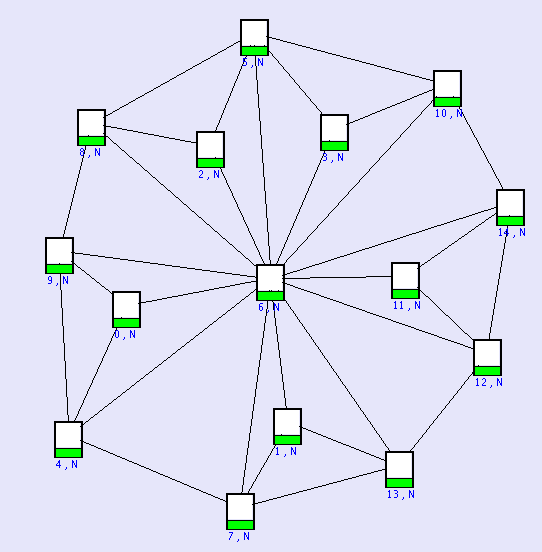
\includegraphics[width=5cm,height=5cm]{images/graphe.png}
  \caption{Exemple de mod�lisation d'un syst�me distribu�}
\end{figure}


\subsection{Communication et Syst�me distribu�}
Dans un syst�me distribu�, la communication peut s'effectuer selon deux modes :
\begin{itemize}
  \item le mode synchrone o� le temps est une donn�e globale du
    r�seau, c'est-�-dire que les (blocs d') instructions de
    l'algorithme s'effectuent sur les tops de l'horloge~;
  \item le mode asynchrone o� les op�rations peuvent se produire �
    n'importe quel instant ind�pendemment de l'ex�cution de celle des
    autres agents.
\end{itemize}

\begin{figure}[ht]
  \centering
  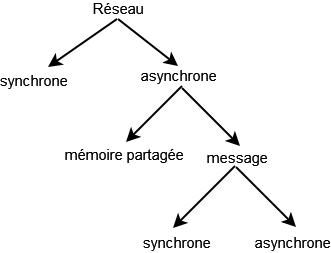
\includegraphics[width=8cm]{images/algodist.png}
  \caption{Les  types  des r�seaux  en  terme  de synchronisation,  un
  sch�ma similaire peut �tre �labor� en s'appuyant sur la connaissance
  ou non des noeuds du r�seau}
  \label{fig:algodist}
\end{figure}

\subsection{Les deux mod�les d'algorithmes}
Il existe deux mod�les d'algorithmes distribu�s :
\begin{itemize}
  \item le mod�le par envoi de messages o� chaque entit�s dispose d'un algorithme qu'elle
  ex�cute et communique avec ses entit�s voisines par l'envoi de message sur le
  r�seau~;
  \item le mod�le avec agent o� les entit�s sont passives, c'est-�-dire
    qu'elles n'effectuent pas de traitement de leur propre initiative,
    les algorithmes sont contenus dans des agents mobiles, qui sont
    des �l�ments poss�dant un algorithme et une m�moire, qui se
    d�placent sur le r�seau et utilisent les sites passifs et leur m�moire pour
    ex�cuter leur algorithme. 
\end{itemize}

\subsection{Probl�mes particuliers � l'algorithmique distribu�e}

\subsubsection{Connaissance partielle}

Une entit� doit faire son calcul avec une connaissance, � priori limit�e, du
syst�me. 
Dans une syst�me non distribu�, l'�tat de la m�moire ne change pas si le processeur ne le modifie pas.
Mais en distribu�, l'entit� ne contr�le que son �tat local. Les donn�es r�parties sur
d'autres unit�s changent sans aucun 
contr�le de de l'entit� consid�r�e.
Parfois l'entit� connait la topologie du graphe en entier, parfois seulement ses
voisins ou ne connait que lui-m�me .

\subsubsection{Terminaison d'un algorithme}

La d�tection de la terminaison d'un algorithme distribu� est souvent difficile,
car elle n�cessite pas seulement d'avoir la connaissance de la terminaison de
son algorithme mais �galement de celle de tous les entit�s  du r�seau.
Nous pouvons cependant chercher �  avoir un d�tection locale de  la terminaison
globale, c'est-�-dire qu'un processeur  peut savoir en fonction de  son �tat et
de celui de ces voisins si l'algorithme est termin�.

\subsubsection{Correction d'un algorithme}

La preuve d'un tel algorithme se fait en deux temps.  Tout d'abord, on
prouve  la   terminaison  de  l'algorithme,   par  des  consid�rations
combinatoires sur le nombre maximum d'�tapes, qui doit �tre fini. Puis
on   prouve   la  validit�,   le   plus   souvent   en  exhibant   des
invariants... sur lesquels on s'appuie pour r�diger la preuve.

\subsubsection{Les erreurs}

Alors qu'en s�quentiel le cas des erreurs est relativement simple: si un �l�ment est
d�fectueux (m�moire, p�riph�rique, 
processeur, disque), on le change et on reprend/continue/recommence le
programme; en distribu�, on peut de plus avoir 
un lien de communication en panne.

Cela peut donc causer de nombreux probl�mes
tels que la corruption des messages 
ou avoir des adversaires qui changent les messages.
Red�marrer tout le syst�me peut parfois �tre �vit� en rendant l'algorithme
robuste (tol�rance aux pannes).

\section{Exemple d'algorithmes distribu�s}

Dans le  domaine de l'algorithmique distribu�e,  de nombreux probl�mes
existent, en voici quelques uns des plus fr�quent.

\subsection{Le probl�me de l'�lection}

\subsubsection*{Principe}
Ce probl�me consiste � distinguer une entit� c'est-�-dire de
l'�lire. La plupart du temps cette �lection permet de s�lectionner une
entit�e pour lui permettre d'acc�der � une ressource critique, les
entit�es non-�lues n'y ayant pas acc�s.

\subsubsection*{Exemple d'Algorithme : Election dans un anneau} 

Soit G un anneau, asynchrone avec �change de messages asynchrones, � 3
�tats :  non �lu,  �lu, ind�fini\\
Les  sommets sont  initialement dans l'�tat   ind�finis.  \\
Chaque processeur i du r�seau poss�de un identificateur   $id_{i}$  unique  (un 
 entier). \\
L'anneau est orient�, c'est-�-dire que les processeurs ont la notion de
gauche et de droite.  \\
Le processeur �lu est celui qui a le plus grand identificateur.  
Chaque processeur transmet � son voisin de droite son
identificateur. \\
Lorsqu'un processeur re�oit  un identificateur, il y a
trois possibilit�s :
\begin{itemize}
\item Si l'identificateur re�u est plus grand que le sien, il le passe
au suivant (voisin de droite) et passe dans l'�tat non �lu.
\item Si l'identificateur re�u est plus petit que le sien, il jette le
message.
\item Si l'identificateur re�u est le m�me que le sien, alors il prend
l'�tat �lu.
\end{itemize}










\subsection{Probl�mes de reconnaissance}

\subsubsection*{Principe}

Peut-on savoir si le r�seau  est un graphe complet, planaire, si c'est
un arbre,  un anneau  ?  Peut-on  savoir encore si  un sommet  est une
articulation, si  une ar�te est un  isthme ?  


\subsubsection*{Exemple 1 d'Algorithme pour le calcul d'un arbre recouvrant}

Cet  algorithme   permet  le   calcul  d'un  arbre   recouvrant  (sans
reconnaissance locale de la  terminaison globale, cf.  algorithme n�2)
. Consid�rons la r�gle de transformation suivante:

\begin{figure}[h!t]
  \centering
  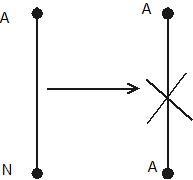
\includegraphics[width=4cm]{images/algodist1.png}
  \caption{Algorithme n�1: Exemple d'une transformation A-N}
  \label{fig:algodist1}
\end{figure}

On  se donne  un graphe  G. Initialement  tous les  sommets  sont dans
l'�tat Neutre.  On choisit  un premier sommet,  dans l'�tat  Actif. On
applique  les transformations  � partir  de ce  point.  Le sous-graphe
d�fini  par les  ar�tes marqu�es  est  un arbre  recouvrant du  graphe
initial.


\subsubsection*{Exemple 2 d'Algorithme pour le calcul d'un arbre recouvrant}

Cet algorithme  permet le calcul d'un arbre  recouvrant avec d�tection
locale de la terminaison globale  (�tat F).  Consid�rons les r�gles de
transformation d�crites  sur la  figure \ref{fig:algodist2} .R1  a une
plus grande priorit� que R2.

\begin{figure}[h!t]
  \centering
  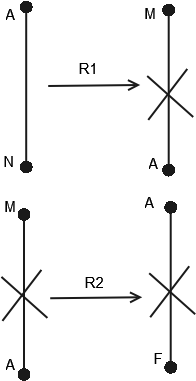
\includegraphics[width=4cm]{images/algodist2.png}
  \caption{Algorithme n�2  : Exemple d'algorithme � base  de r�gles de
  r��critures}
  \label{fig:algodist2}
\end{figure}




\section{Quelques applications}

L'algorithmique distribu�e est appliqu� dans plusieurs domaines, comme
par exemple :
\begin{itemize}
  \item Construction d'objets parall�les : Un exemple des applications dans ce
  		domaine est men� par le PRISM
		\footnote{le laboratoire  de recherche en informatique  sur les th�mes
		du Parall�lisme, des R�seaux, des Syst�mes et de la Mod�lisation.(voir
		http://www.prism.uvsq.fr/)}, il consiste dans la construction d'objets
		pour  l'�laboration d'algorithmes  d'alg�bre lin�aire  utilisables par
		des architectures � m�moire distribu�e. 
 \item  Le domaine de l'�nergie : Un  exemple  d'application  dans  ce  domaine 
		on le  trouve  au  LAG \footnote{le Laboratoire    d'Automatique    de  
		Grenoble    (voir
		http://www.lag.ensieg.inpg.fr/)}  ,  et  qui  vise  contrairement  aux
		approches  traditionnelles  qui  consistent  � ajuster  la  production
		d'�nergie pour  satisfaire �  la demande, �  proposer un  m�canisme de
		coop�ration entre sources et charges  de fa�on � satisfaire au mieux �
		des crit�res de satisfaction d�finis par un usager.  
\end{itemize}





\chapter{Analyse de l'existant}
\section{Pr�sentation de \visidia}

\subsection{L'application}

Avec la g�n�ralisation des r�seaux tels qu'Internet et le d�veloppement d'une
information de plus en plus complexe et massivement distribu�e sur ses grands
r�seaux, de nombreuses applications industrielles, banquaires et web sont elles
aussi devenues distribu�es.\\

Toutefois, le d�veloppement d'applications distribu�es est un processus tr�s difficile.
� la complexit� classique de d�veloppement d'applications centralis�es, s'ajoute une complexit� 
li�e � la distribution et � l'introduction de la communication entre processus, de la concurrence,
des conflits de ressources.  \\

C'est dans ce cadre, que les chercheurs du LaBRI ont lanc� le projet \visidia
\footnote{\url{http://www.labri.fr/projet/visidia}}.
\visidia se propose de fournir un atelier compos� d'outils de simulation, de
visualisation et d'aide aux preuves devenus indispensables pour la conception,
les tests et la validation de programmes dans des environnements distribu�s. Le mod�le
classique consiste � repr�senter le r�seau par un graphe o� les 
sommets correspondent � des machines ou processeurs, et les ar�tes � des
connexions. \\ 

\begin{figure}[H]
  \centering
  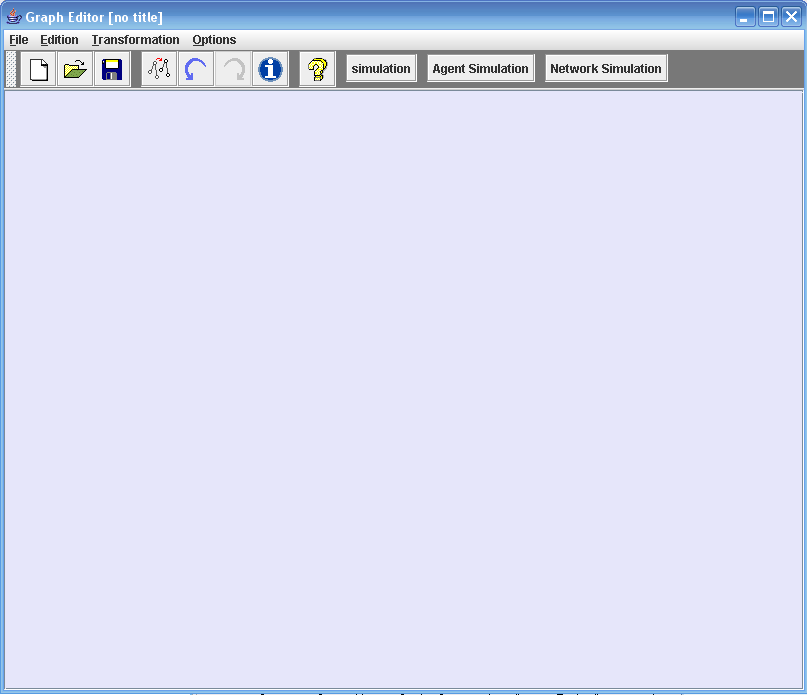
\includegraphics[width=6cm]{images/visidia_general.png}
  \caption{L'application Visidia}
  \label{fig:implantation-communication}
\end{figure}

\visidia impl�mente les deux mod�les d'algorithmes distribu�s, la version avec
envoi de messsages, et celle � base d'agents mobiles.
Nous nous int�resserons seulement � la simulation avec les agents mobiles
durant ce projet.



\subsection{La simulation avec agents mobiles}

Le dev�loppement de l'application est articul� autour d'une s�paration de
l'architecture en trois parties, totalement ind�pendantes,  et communiquant
entre elles par l'envoi de messages :
\begin{itemize}
  \item Simulation 
  \item Affichage
  \item Algorithmes ou agents mobiles
\end{itemize}


\begin{figure}[H]
  \centering
  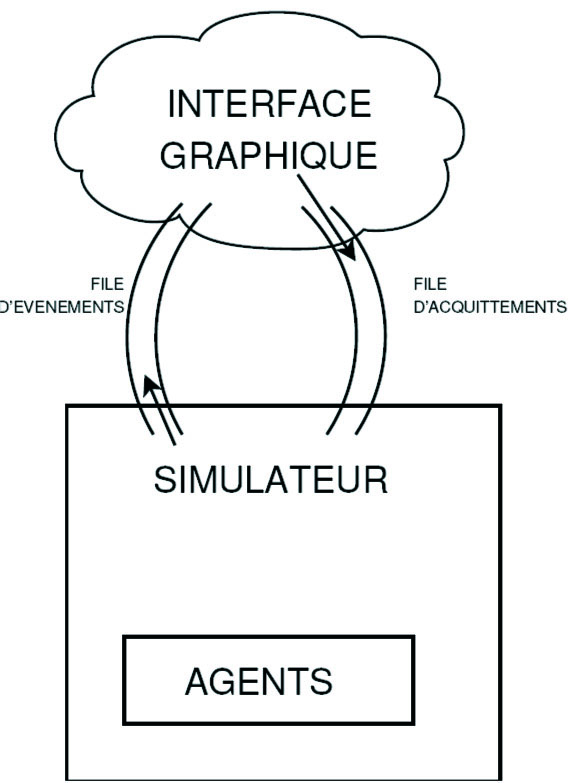
\includegraphics[width=6cm]{images/structureVisidia.png}
  \caption{Structuration de \visidia}
  \label{fig:implantation-communication}
\end{figure}


\begin{figure}[H]
  \centering
  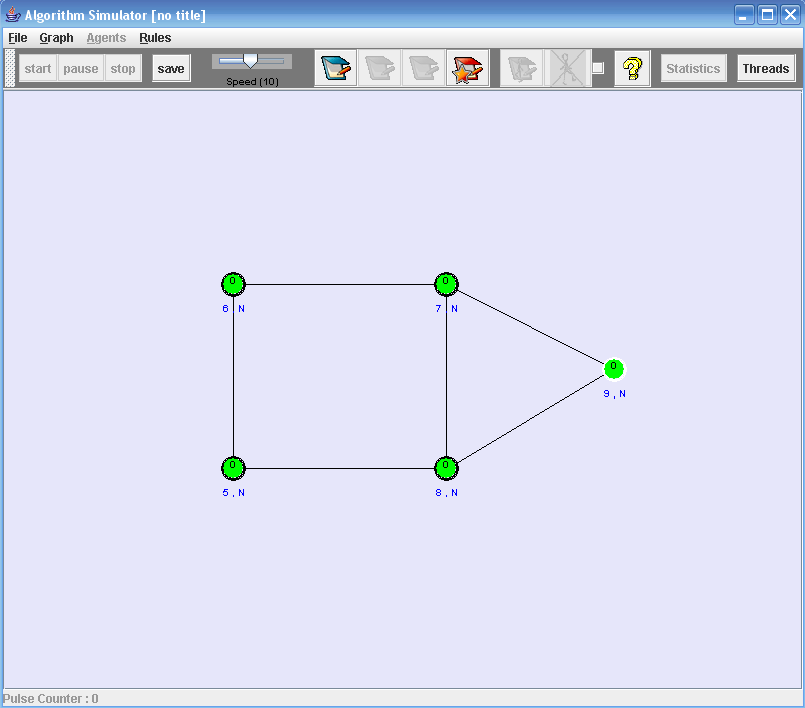
\includegraphics[width=6cm]{images/visidia_agents.png}
  \caption{Simulation avec agents mobiles}
  \label{fig:implantation-communication}
\end{figure}



Dans la version de base qui nous a �t� fournie, on a d�j�
une impl�mentation de la simulation d'algorithmes avec agent
mobile. Celle-ci s'appuie sur la version initiale travaillant par
envoi de message : c'est pourquoi cela apporte des contraintes
suppl�mentaires, notamment au niveau de la partie graphique.\\

L'utilisateur a d�j� la possibilit� de cr�er un graphe,
d'ouvrir un graphe et de sauvegarder un graphe. Ensuite, le choix se
porte sur le type d'algorithme � ex�cuter : une version par envoi
de messages et une version avec agents mobiles. Nous ne traiterons que
cette derni�re version.\\

Apr�s avoir s�lectionn� l'ex�cution d'algorithme avec
agents mobiles, l'utilisateur arrive dans la fen�tre de
simulation. Il lui est d�j� possible, avant tout lancement
d'ex�cution d'algorithmes, d'ajouter diff�rents types d'agent
sur le graphe. Par contre, � ce stade, il est impossible de
modifier le graphe sans fermer la fen�tre de simulation. Enfin, une
fois la simualtion lanc�e, il est �galement impossible de
supprimer un agent ou d'en ajouter, de modifier le graphe pendant une
ex�cution ou encore de connaitre des statistiques en temps
r�el : le but du projet est d'ajouter entre autres ces
fonctionnalit�s.



\section{L'aspect technique}

\subsection{Code source}

Nous avons r�cup�r� la derni�re version de d�veloppement de \visidia. Celle-ci
est disponible sur notre svn : 
\begin{verbatim}
svn checkout svn://svn.berlios.de/visidia/trunk
\end{verbatim}

Le code source de \visidia est parfois comment� avec l'outil \textbf{javadoc}. \\
Tr�s peu de classes et d'attribut ont �t� comment�s.

\subsection{Documentation}

La documentation qui nous a �t� fournie a �t� le rapport de
PFA de l'�quipe pr�c�dente.\\
Nous n'avons pas eu connaissance de l'existance d'un rapport technique
expliquant les principes techniques de d�veloppement de l'application depuis son
d�but.

\chapter{Expression du besoin}
Dans cette partie, nous allons d�crire les besoins fonctionnels li�s au projet 
(ajout de nouvelles fonctionnalit�s, modification de l'interface) ainsi que les 
besoins non fonctionnels (langage, licence, etc.) li�s au projet.

\section{Besoins fonctionnels}

Nous d�crivons ici les nouvelles fonctionnalit�s du logiciel \visidia. 
Nous nous attarderons simplement � d�tailler les entr�es et sorties de chaque 
nouvelle fonctionnalit�, sans aborder l'impl�mentation (qui fera l'objet du prochain 
chapitre portant sur l'impl�mentation). Les sp�cifications des besoins fonctionnels 
d�crivent le nouveau comportement externe du logiciel \visidia.


\subsection{Mise en pause du programme}
Cette fonctionnalit� �tait d�j� pr�sente dans le
logiciel au d�but du projet : l'appui sur un bouton de mise en
pause interrompt tous les agents en cours d'ex�cution. Cependant
cette fonctionnalit�, n�cessaire lors d'une modification sur un
agent ou sur le graphe pendant la simulation (c'est-�-dire pendant
l'ex�cution), est devenue compl�tement transparente pour
l'utilisateur. Ce dernier n'a pas besoin de mettre en pause le
programme lors d'une modification dans la fen�tre de simulation.\\

\begin{itemize}
  \item Entr�e : modification (sur un agent ou sur le graphe) pendant la simulation
  \item Sortie : mise en pause automatique, modification apport�e, simulation
  toujours en cours d'ex�cution 
\end{itemize}


\subsection{Modification de la m�moire d'un sommet}
Pendant l'ex�cution d'un algorithme avec agents mobiles, l'utilisateur peut
modifier l'�tat de la m�moire d'un sommet. L'utilisateur s�lectionne le sommet
dont il souhaite modifier la m�moire : il peut alors consulter sa m�moire puis
la modifier pendant l'ex�cution de l'algorithme.\\

\begin{itemize}
  \item Entr�e : s�lection d'un sommet
  \item Sortie : apr�s consultation de l'�tat de la m�moire du sommet,
  modification de la m�moire du sommet 
\end{itemize}


\subsection{Extinction et allumage d'un sommet}
Pendant l'ex�cution d'un algorithme avec agents mobiles,
l'utilisateur peut �teindre un sommet : celui-ci fait toujours
partie du graphe, mais il est \textit{�teint}. Les sommets voisins
du sommet �teint n'envoient alors plus d'agents mobiles vers ce
sommet tant que celui-ci ne sera pas \textit{rallum�}. Si un agent
a d�j� �t� envoy� vers ce sommet �teint (lors de
l'extinction, l'agent se trouve sur une ar�te incidente), alors
l'agent est renvoy� vers le sommet dont il provient.\\

\begin{itemize}
  \item Entr�e : s�lection d'un sommet allum�
  \item Sortie : sommet �teint ne traitant plus les agents\\
\end{itemize}

Pendant l'ex�cution d'un algorithme avec agents mobiles,
l'utilisateur peut allumer un sommet �teint : cette action est
compl�mentaire � l'extinction d'un sommet. Un sommet �teint
peut �tre rallum�, c'est-�-dire que ce sommet devient comme
initialement parfaitement fonctionnel.\\ 

\begin{itemize}
  \item Entr�e : s�lection d'un sommet �teint
  \item Sortie : sommet allum� traitant � nouveau les agents
\end{itemize}


\subsection{Ajout et suppression d'un sommet}
Pendant l'ex�cution d'un algorithme avec agents mobiles,
l'utilisateur peut ajouter un sommet. Cette action peut s'effectuer
plusieurs fois de suite, sans que le programme soit mis en pause.\\ 

\begin{itemize}
  \item Entr�e : s�lection d'une zone o� ajouter un sommet
  \item Sortie : sommet ajout� pendant l'ex�cution de l'algorithme\\
\end{itemize}

Pendant l'ex�cution d'un algorithme avec agents mobiles,
l'utilisateur peut supprimer un sommet. Toutes les ar�tes
incidentes au sommet sont �galement supprim�es. Si un agent est
pr�sent sur le sommet lors de la suppression, alors il est
tu�. Si un agent est pr�sent sur une des ar�tes supprim�es, alors
celui-ci n'est tu� que s'il arrive sur le sommet supprim�.\\ 

\begin{itemize}
  \item Entr�e : s�lection d'un sommet � supprimer
  \item Sortie : sommet supprim� ainsi que toutes les ar�tes qui lui sont incidentes
\end{itemize}


\subsection{Ajout et suppression d'une ar�te}
Pendant l'ex�cution d'un algorithme avec agents mobiles, l'utilisateur peut
ajouter une ar�te. L'ajout d'ar�te s'effectue entre deux sommets d�j� pr�sents,
par un \textit{glisser-d�placer} avec clic gauche de la souris.\\

\begin{itemize}
  \item Entr�e : s�lection du premier sommet, puis \textit{glisser-d�placer}
  vers le second sommet 
  \item Sortie : ar�te ajout�e entre les deux sommets\\
\end{itemize}


Pendant l'ex�cution d'un algorithme avec agents mobiles, l'utilisateur peut
supprimer une ar�te. Il suffit de s�lectionner l'ar�te � supprimer et d'activer
le bouton ad�quat. Si un agent est pr�sent sur l'ar�te en cours de suppression,
celui-ci est tu�.\\

\begin{itemize}
  \item Entr�e : s�lection d'une ar�te � supprimer
  \item Sortie : ar�te supprim�e
\end{itemize}


\subsection{Ajout et suppression d'un agent}
Pendant l'ex�cution d'un algorithme avec agents mobiles, l'utilisateur peut
ajouter un agent. Apr�s avoir s�lectionn� le sommet o� ajouter l'agent,
l'utilisateur choisit ensuite le type d'agent qu'il souhaite ajouter.\\

\begin{itemize}
  \item Entr�e : s�lection d'un sommet o� ajouter un agent
  \item Sortie : apr�s s�lection du type d'agent, ajout de l'agent sur le
  sommet et ex�cution de son algorithme\\
\end{itemize}

Pendant l'ex�cution d'un algorithme avec agents mobiles, l'utilisateur peut
supprimer un agent. L'utilisateur active le bouton permettant la suppression
d'agent : il s�lectionne ensuite le nom de l'agent qu'il d�sire supprimer. Ce
dernier sera alors d�finitivement supprim� de la simulation.\\

\begin{itemize}
  \item Entr�e : activation du bouton de suppression d'agents
  \item Sortie : apr�s s�lection du nom de l'agent, suppression d�finitive de
  l'agent dans la simulation
\end{itemize}


\subsection{Modification de la m�moire d'un agent}
Pendant l'ex�cution d'un algorithme avec agents mobiles, l'utilisateur peut
modifier la m�moire d'un agent. L'utilisateur active le bouton de consultation
des m�moires des agents. Apr�s avoir s�lectionn� l'agent � consulter,
l'utilisateur active le bouton de modification de sa m�moire : il s�lectionne
ensuite le champ � modifier et entre une nouvelle valeur.\\

\begin{itemize}
  \item Entr�e : activation du bouton de consultation de la m�moire des agents
  \item Sortie : apr�s s�lection du nom de l'agent puis du champ � modifier, la
  nouvelle valeur est entr�e dans la m�moire de l'agent
\end{itemize}


\subsection{Statistiques}
Pendant l'ex�cution d'un algorithme avec agents mobiles, l'utilisateur peut
afficher en temps r�el des statistiques par agent et des statistiques sur
l'ex�cution d'un algorithme. Entre autres, on peut conna�tre le nombre de pas
effectu�s par chaque agent, par chaque classe d'agent (nombre moyen de pas,
nombre minimum, maximum), la taille de la m�moire, etc.\\

\begin{itemize}
  \item Entr�e : activation du bouton de consultation des statistiques
  \item Sortie : affichage des statistiques en temps r�el sur l'algorithme en cours d'ex�cution
\end{itemize}


\section{Besoins non fonctionnels}

\subsection{Impl�mentation d'algorithmes distribu�s}
Plusieurs nouveaux algorithmes ont �t� impl�ment�s, dans le but d'enrichir la
biblioth�que d'algorithmes disponibles et afin de valider le travail r�alis�.\\


\begin{itemize}
  \item Fusion des m�moires : dans cet algorithme, les agents se d�placent de
  mani�re synchrone. Ils se rencontrent sur les sommets (o� ils ont le choix de
  rester sur place ou de se d�placer au prochain \texttt{top}), l'agent dont
  l'identificateur est le plus grand r�cup�re la m�moire des autres agents du
  m�me type pr�sents sur le sommet et les autres agents sont tu�s.
  \item Calcul d'arbre recouvrant avec plusieurs agents.
  \item Algorithme fourni par M. Hamid (algorithme auto-stabilisant
  avec des agents sur un anneau).
\end{itemize}


\subsection{Structuration de l'application}
Le d�veloppement de nouvelles fonctionnalit�s au logiciel \visidia s'est
effectu� en respectant la s�paration en trois modules : l'interface graphique,
le simulateur et les agents.


\subsection{Langage et portabilit�}
Les standards de codage d�finis par le langage Java ont �t� utilis�s : un
reformatage des sources dans ce sens a d'ailleurs �t� effectu�.
L'interface en anglais a �t� conserv�e. Le logiciel \visidia n�cessite toujours
une version du JDK sup�rieure ou �gale � la version 1.5.


\subsection{Documentation sur l'impl�mentation de nouveaux agents mobiles}
Une documentation concernant comment impl�menter de nouveaux algorithmes avec
agent mobile a �t� r�alis�e. Celle-ci facilitera la t�che d'impl�mentation en
vue d'enrichir la biblioth�que d'algorithmes existants.


\chapter{Travail r�alis�}
\section{Ajout de fonctionnalit�s}

\subsection{Modification du graphe en cours d'ex�cution}

\subsection{Structure du graphe}

Dans visidia, il y a une s�paration totale entre la partie affichage et la
partie simulation. Ainsi, \visidia manipule deux graphes : un graphe visuel et un
autre pour la simulation.\\

N'ayant aucune indication sur les structures de ces graphes, on pouvait imaginer
que les structures de ces graphes pouvaient �tre les m�mes, ou bien avoir des
points en commun.\\

Apr�s une analyse plus pouss� du code, nous avons d�couvert que les deux
structures �taient totalement dissoci�s et ind�pendante l'une de l'autre.
Pour la partie simulation, le r�pertoire ``graph'' contient toutes les classes
de l'architecture du graphe.
%inclure sch�ma architecture

Pour la partie affichage, le repertoire ``gui.presentation'' contient les
classes impl�mentant la structure du graphe visuel.


\subsection{Choix de d�veloppement}

Lors de la conception de \visidia, il n'a pas �t� pr�vu que le graphe visuel
puisse �voluer au cours de la simulation.
En effet, aucune int�raction entre les deux graphes n'a �t� envisag�s hormis, la
conversion d'un graphe visuel en un graphe de simulation par l'interm�diaire de
la classe ``Convertisseur''et de sa m�thode ``convert".\\

En effet, le graphe visuel dessin� dans l'application principale est converti
un graphe simulation au moment du passage vers l'application ``simulation avec
agents''. 
Apr�s cette manipulation le graphe visuel �tant pr�sum� statique, aucune m�thode
agissant sur le graphe dessin�, ne r�percutait les modifications sur le graphe de
simulation et vice versa.\\

Une solution possible � laquelle nous avions pens�, et qui permettait de
r�utiliser ce qui avait �t� d�velopp� jusqu'� pr�sent, �tait de
convertir le graphe visuel vers un graphe simulation � chaque fois que l'on
modifiait le graphe visuel. 
Nous n'avons cependant pas choisi d'impl�menter cette m�thode pour des raisons
�videntes de performance: la g�n�ration d'un nouveau graphe de simulation �
chaque ajout ou suppression d'aretes ou sommet peut s'averer tres couteux,
surtout avec un graphe de grande taille. \\

Ainsi donc nous avons pr�f�r� pour chaques modifications possible sur le graphe visuel, 
impl�menter une m�thode permettant de r�percuter les effets sur le graphe de simulation.

\subsection{Ajout de sommets et d'aretes}



\subsection{Suppression de sommets et d'aretes}






\subsection{Ajout - Suppresion d'agent en cours d'ex�cution}



\subsection{Modification des whiteboards}



\subsection{Calcul de statistiques}



\section{Impl�mentation d'algorithmes}



\chapter{Limites et extension du projet}
\section{Les limites du projet}

Au cours de ce projet, la principale limite � laquelle nous avons �t� confront�s
est le manque de documentation technique pr�cise et compl�te sur l'application.\\

Nous avons donc du souvent passer beaucoup de temps pour comprendre ce que
r�alisait une classe, une m�thode, le r�le d'un attribut, ma�triser les principes
fondamentaux sur lesquels reposent \visidia.


\section{Extension du projet}

Une fonctionnalit� qu'il serait utile de rajouter � \visidia serait de faire une
totale s�paration, entre l'algorithme ex�cut� par l'agent, et son algorithme de
d�placement.\\

Une autre �volution envisageable consisterait � d�velopper un
applet java afin de pouvoir utiliser 
l'application � l'aide d'un simple navigateur internet.\\

Il pourrait �tre int�ressant �galement de r�aliser de la simulation
d'algorithmes distribu�s sur de vrais r�seaux de machines physiques. \\


\chapter{Organisation du projet}

\section{Les moyens techniques}

Afin de mener � bien notre projet, nous avons utilis�s un portail �volu� de
d�veloppement fournissant plusieurs outils : le portail berliOs.de \footnote{\url{http://www.berlios.de}}
\\ \newline
Pour am�liorer la communication avec notre client et notre responsable
p�dagogique, nous avons mis en place un wiki sur lequel on pouvait retrouver
toutes les principales informations relatives au projet.\\

\begin{figure}[H]
  \centering
  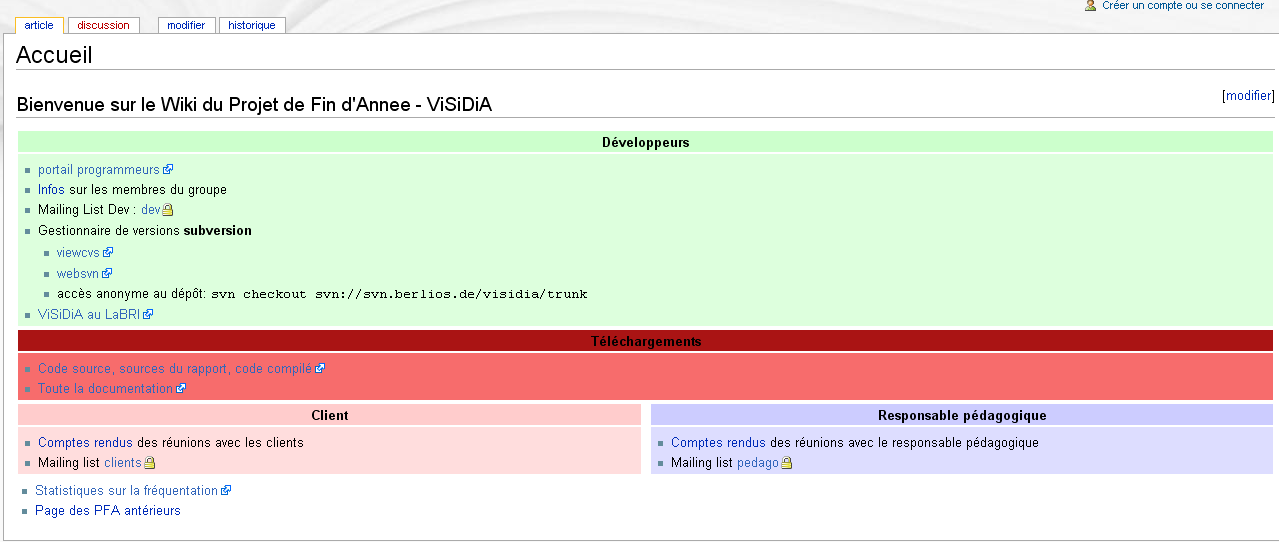
\includegraphics[width=16cm]{images/wiki.png}
  \caption{Le wiki du projet Visidia}
\end{figure}

Nous avons d�ploy�s plusieurs listes de diffusion pour faciliter la communication :
\begin{itemize}
  \item Une liste pour tous les d�veloppeurs
  \item Une liste de diffusion pour communiquer avec le client
  \item Une liste de diffusion pour communiquer avec le responsable p�dagogique \\
\end{itemize}

Nous avons utilis� �galement un gestionnaire de versions, Subversion
, qui nous permet de maintenir les sources de \visidia. 
Les clients ont �galement la possibilit� de
suivre l'avancement du projet et d'acc�der aux sources, gr�ce � deux
interfaces viewcvs  et websvn .  Il est
�galement possible de t�l�charger la derni�re version des sources du
projet:
\begin{verbatim}
svn checkout svn://svn.berlios.de/visidia/trunk
\end{verbatim}


\section{Organisation du travail}

Notre groupe de travail �tant form� de 6 personnes, nous avons d�cid�s de former
trois bin�mes afin de favoriser et optimiser le travail en �quipe. 
De plus la formation de binome permettait de mettre en place le systeme
d�veloppeur/relecteur, et facilite l'appr�hension d'une application comme
\visidia, puisque chacun pouvait expliquer � son partenaire les concepts qu'il avait
saisi pour mututellement enrichir ses connaissances de l'application.\\

Nous nous sommes r�parti le travail de mani�re � faire en sorte, que les binomes
form�s n'ait � se concentrer essentiellement que sur une partie du d�veloppement
de \visidia. Ainsi nous avons eu un binom� charg� d'impl�menter les
fonctionnalit�s relatives aux graphes et un autre celles relatives aux agents.

\section{Avancement du projet}

\begin{figure}[!ht]
  \center
  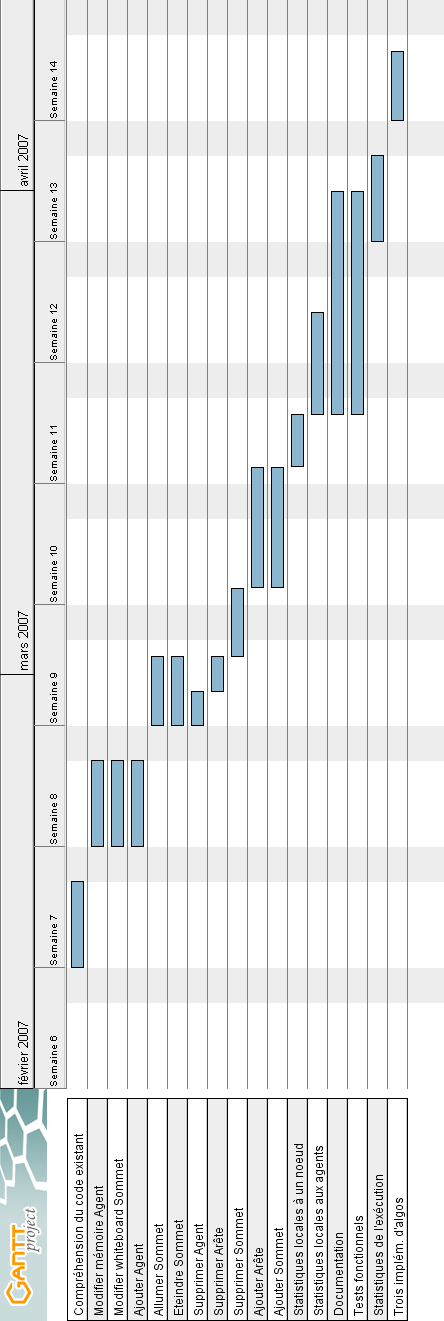
\includegraphics[height=20cm]{images/gantt2.png}
  \caption{Diagramme de Gantt}
\end{figure}
%diagramme de gant a mettre la




\chapter*{Conclusion}
\addcontentsline{toc}{chapter}{Conclusion}
Les fonctionnalit�s demand�es par le client dans le cahier des charges ont �t�
toutes d�velopp�es. Nous avons �galement r�ussi � impl�menter le nombre voulu
d'algorithmes. Nous avons aussi, dans la mesure possible, essay� de d�velopper les
fonctionnalit�s suppl�mentaires souhait�es. N�anmoins, une documentation plus
fournie aurait facilit� la compr�hension du code. Nous avons donc pr�t� une
attention particuli�re � la documentation du travail que nous avons r�alis�.\\

Ce projet a �t� l'occasion de pouvoir approfondir nos connaissances en java,
et plus particuli�rement les fonctionnalit�s d'acc�s concurent et de gestion
des threads. 
L'impl�mentation des agents nous a confront� � des situations de calcul
distribu� complexe o� l'information connue se limite � celle de l'agent et du
sommet o� il se trouve.
L'exercice de reprise de code existant a �t� difficile � appr�hender. Il nous a
�t� toutefois b�n�fique d'y �tre confront� car nous seront s�rement amen� � le
rencontrer souvent en entreprise.\\

L'algorithmique distribu� �tant de plus en plus utilis� dans les syst�mes
informatique, ce projet a �t� l'occasion d'acqu�rir une exp�rience sur cette technologie.


\chapter*{Annexe}
\addcontentsline{toc}{chapter}{Annexe}
  %\begin{verbatim}
/**
* Implements the rendez-vous algorithm ; memories of the agents are merged when
* they meet : only the agent with the best ID is not killed
*/
public class RdvSynchronizedAgent extends SynchronizedAgent {

  protected void init() {
    /* Memory of the agent that will be fusionned with the
     * other agents */ 
    this.setProperty("myName", "a" + this.getIdentity());
    
    /* Agent move method */
    this.setAgentMover("RandomAgentMover");
    
    /* Random Class to know whether to move the agent or
     * not (if not, the agent remains on its vertex). The
     * algorithm makes the hypothesis that an agent has
     * the choice to remain on a vertex  */
    Random rnd = new Random();
    
    int agentId = this.getIdentity();
    
    /* The algorithm ends when the total number of
     * 'RdvSynchronizedAgent' on the graph is equal to 1 */  
    while (! oneAgentRdvRemaining()) {
      
      
      /* Puts its ID on the vertex if it is better */
      this.lockVertexProperties();
      try {
	Integer currentBestId = (Integer) this.getVertexProperty("maxId");
	if (agentId > currentBestId.intValue()){
	  this.setVertexProperty("maxId", new Integer(agentId));
	}
      } catch (NoSuchElementException e){
	this.setVertexProperty("maxId", new Integer(agentId));
      }
      this.unlockVertexProperties();
      
      this.nextPulse();
      
      

      /* If 'maxId' on the vertex is better than its ID,
       * it puts its memory on the vertex and then kills itself */
      if (agentId < ((Integer) this.getVertexProperty("maxId")).intValue()){
	fusionAgentToVertex(this);
	return;  /* Kills itself */
      }
      
      this.nextPulse();


      /* If here, the agent 'this' has the better ID on the vertex :
       * it adds to its memory the whiteboard of the vertex on which
       * it is */ 
      String currentFusion = "";
      try {
	currentFusion = (String) this.getVertexProperty("fusion");
	if (! (currentFusion.length() == 0)){
	  this.setProperty("myName", this.getProperty("myName") + " " + ((String) this.getVertexProperty("fusion")));
	}
      } catch (NoSuchElementException e){
	this.setVertexProperty("fusion", "");
      }


      /* Erase the memory of the vertex (memory of the agent in
       * 'fusion' and 'maxId') */
      this.lockVertexProperties();
      this.setVertexProperty("fusion", "");
      this.setVertexProperty("maxId", new Integer(0));
      this.unlockVertexProperties();


      /* Move the agent to a next vertex with a chance of 1 out of 3 */ 
      int choice = rnd.nextInt() % 2;

      if (choice == 0){
	this.move();
      }
      this.nextPulse();

    }
  }




  /**
  * This function returns true if it remains exactly one agent of type
  * RdvSynchronizedAgent on the graph, false otherwise
  */
  private Boolean oneAgentRdvRemaining(){
    Collection allAgents = this.getSimulator().getAllAgents();

    if (! allAgents.isEmpty()){
      Iterator it = allAgents.iterator();
      while(it.hasNext()){
	Agent currentAgent = (Agent) it.next();
	/* Try to find an agent of the same class with a different ID */
	if((currentAgent.getClass() == this.getClass()) && (currentAgent.getIdentity() != this.getIdentity())){
	  return false;
	}
      }
      /* The agent didn't find any other agent of its class  : it is
       * the only one remaining on the graph */
      return true;
    } else {
      return false;
    }
  }




  /**
  * This function adds the agent memory to the whiteboard of the
  * vertex on which the agent is
  */
  private void fusionAgentToVertex(Agent agent){
    String agentName = (String) this.getProperty("myName");
    this.lockVertexProperties();
    String currentFusion = "";
    try {
      currentFusion = (String) this.getVertexProperty("fusion");
    } catch (NoSuchElementException e){
      this.setVertexProperty("fusion", currentFusion);
    }
    this.setVertexProperty("fusion", currentFusion + " " + agentName);
    this.unlockVertexProperties();
  }

}
\end{verbatim}


\end{document}
